\cotefile{31}
\scanpage{2}
\uline{$\mathrm{cd}^{\unsure{!|'}}_{\ell}(k)$ \unsure{pour} $k$ de}
\uline{\unsure{car.} $p$.}

(\unsure{dualité} \unsure{glob})

\margin{\unsure{4}}
\margin{\unsure{1}}

\scanpage{3}
$k$ corps de \unsure{car.} $p>0$

On désigne par $\mathrm{cd}_p(k)$ la dimension cohomologique,
\unsure{calculée} pour les faisceaux de $p$-torsion pour la
topologie finie \deleted{\unsure{étale}} \inserted{fid. plate} sur $k$. Regardons d'abord
le $\mathrm{cd}'_p(k)$, \unsure{calculée} avec des groupes algébriques
\inserted{(\unsure{comm.})} finis sur $k$, \inserted{d'ordre une puiss. de $p$.} Tout tel groupe algébrique se \unsure{dévisse}
en
\[
G'\subset G''\subset G
\]
où $G''=G^0$ et $G/G''$ est un groupe
étale, et où $G'$ est \inserted{(radiciel)} de t. un. tandis
$G''\unsure{/|\ne}G'$ \inserted{(radiciel)} de type multiplicatif. Donc

\uline{Lemme 1} $\mathrm{cd}'_p(k)\leq n\Longleftrightarrow H^i(k,G)=0$ pour $i>n$,
lorsque $G$ est \inserted{un groupe fini sur $k$ de} l'un des types suivants:

a) $G$ étale sur $k$ ; \quad [i.e. \deleted{$\unsure{\Longleftrightarrow}$} $\mathrm{cd}^{\text{ét}}_p(k)\leq n$]

b) $G$ \unsure{radiciel} et t. un. sur $k$

c) $G$ est radiciel et t. multiplicatif.

\margin{2}

\scanpage{4}
est toujours vérifiée si $G$ est un tore). Alors la démonstration donnée
montre que dans l'énoncé de 4.6. \inserted{et les corollaires 4.7. et 4.8. ,} on peut se borner à considérer les
sous-groupes de la forme ${}_{m^r}G$, avec $r\quad 0$. D'ailleurs, on voit \unsure{aussitôt}
\deleted{que} \inserted{lorsque $G$ est \uline{simple} sur $S$, alors} pour tout point $s\quad S$, il existe un voisinage ouvert $U$ de $s$ \deleted{tel}
et un entier $m\quad 0$, premier à toutes les caractéristiques \deleted{\unsure{résiduelles}}
résiduelles de $U$, et qui satisfait les conditions précédentes pour $G\quad U$.
(Prendre par exemple pour $m$ l'ordre de la torsion du type de $\unsure{G|H}$ \deleted{dans}
en $s$). Sous ces conditions, on trouve des ${}_{m^r}G$ qui sont finis et
\uline{étales} sur $S$, et dont la famille est schématiquement dense, à condition
de se restreindre au dessus de $U$. Cette remarque permet dans certains
cas (notamment \deleted{\unsure{dans l'application}} \inserted{ceux faisant intervenir} des théorèmes 3.2. et 3.2. bis, cf
\inserted{Appendice -}
mais non celle des théorèmes 3.6. et 3.6. bis) de se passer du théorème 3.1. faisant intervenir la cohomologie de Hochschild. \deleted{Bien
entendu, la remarque \unsure{analogue} s'applique aux deux corollaires 4.7. et
4.8.}

5. \uline{Homomorphismes centraux des groupes de type multiplicatif}.

\uline{Théorème} 5.1. Soient $u,v:H\quad G$ deux homomorphismes de $S$-préschémas en groupes, avec $H$ de type multiplicatif et de type fini; \deleted{On
suppose} $G$ de présentation finie sur $S$, \deleted{ou $S$ localement noethérien.}
Soit $s\quad S$ tel que $u_s=v_s$, et supposons $u$ \uline{central}. Alors il existe
un voisinage ouvert $U$ de $s$ tel que $u_U=v_U$.

Distinguons les deux cas: a) $S$ localement noethérien, auquel cas
on peut se borner à supposer $H$ localement de type fini sur $S$. Cette
dernière hypothèse et EGA IV 8 nous permettent de remplacer $S$ par
le spectre de $\underline{O}_{S,s}$, donc de supposer $S$ local de point fermé $s$. Quitte
à remplacer l'anneau local $A$ par son complété, ce qui introduit un
changement de base fidèlement plat et quasi-compact, on peut même supposer $A$ complet. En vertu de 3.4. on aura $u_n=v_n$ pour tout $n$,

\margin{3}

\scanpage{5}
Noter que $\mathrm{cd}^{\text{ét}}_p(k)$ est égal à $0$ ou $1$, suivant
que \deleted{toute} extension \inserted{\figure{\begin{tikzpicture}[baseline=(n.base)]\node[draw,ellipse,inner sep=1pt] (n) {finie};\end{tikzpicture}}} étale de $k$ est d'ordre
premier à $p$, ou non.

Si $G$ est de t. m., alors $G$ est dual
d'un groupe fini étale $C$ lequel est
quotient d'un module galoisien, \unsure{libre} de
type fini sur $\mathbf{Z}$, donc $G$ est contenu
dans un tore, donc on a une suite
exacte
\diagram{\begin{tikzcd}
0\arrow[r]&G\arrow[r]&T\arrow[r]&T'\arrow[r]&0
\end{tikzcd}}
$T$ et $T'$ des tores. D'où le

\uline{Lemme 2} Pour que $\mathrm{cd}^{\text{t.m.}}_p(k)$ soit $\leq n$,
\margin{$\left[\rule{0pt}{6em}\right.$}
il f. et s. que les conditions suivantes
soient vérifiées: pour tt tore $T$ sur $k$,
$H^i(k,T)(p)$ est nul pour $i>n$, et $p$-divisible
si $i=n$.
\inserted{[Ou encore: pour tte extension finie \unsure{sép.} $k'$ de $k$ [\unsure{il suffit} d'ordre premier à $p$]
\deleted{$\operatorname{Br}(k)(p)$} $H^i(k',G_m)=0$ \inserted{si $i>n$, et $H^{\unsure{n}}(k',G_m)$ est $p$-divisible}]}

Comme on a
\diagram{\begin{tikzcd}
0\arrow[r]&{}_{p}T\arrow[r]&T\arrow[r,"p"]&T\arrow[r]&0
\end{tikzcd}}
d'où
\[
\deleted{\left\{ {}_{p}H^{\unsure{i|n}}(T)=\operatorname{Im}H^i({}_{p}T)\right.}
\]
\margin{4}

\scanpage{6}
ou comme d'habitude l'indice $n$ indique la réduction mod \deleted{la puissance}
$\underline{m}^{n+1}$ ($\underline{m}$ étant l'idéal maximal de $A$). Pour tout entier $m\quad0$, dénotant
par ${}_m u,{}_m v$ les homomorphismes ${}_m H\quad G$ induits par $u,v$, on aura donc
aussi $({}_m u)_n=({}_m v)_n$. Ceci étant vrai pour tout $n$, et ${}_m H$ étant \uline{fini}
sur $S$ en vertu de 2.2. , il s'ensuit qu'on aura ${}_m u={}_m v$. Ceci étant
vrai pour tout $m$, on aura $u=v$ en vertu de 4.7. a).

b) Cas général. Nous \deleted{\unsure{supposerons}} pouvons supposer $S$ \deleted{local
\unsure{de point fermé $s$.}} \inserted{affine, $S=\operatorname{Spec}(A)$.} Quitte à faire une extension fidèlement plate et quasi-compacte de la base, on peut supposer de plus $H$ diagonalisable, donc
de la forme $D_S(M)$, avec $M$ un groupe commutatif de type fini. Introduisons comme dans la démonstration de 4.6. la famille filtrante croissante des sous-$\underline{Z}$-algèbres \deleted{$A_i$} de type fini $A_i$ de $A$. Comme $G$ est de présentation finie sur $S$, il provient d'un \deleted{schéma} préschéma en groupes de
présentation finie $G_i$ sur un $S_i$. D'ailleurs, $H$ provient de $H_i=D_{S_i}(M)$.
De plus, pour $j$ grand, en vertu de EGA IV 8, les homomorphismes
\deleted{$u,v$} $u,v$ proviennent d'homomorphismes de $S_j$-groupes \deleted{$\unsure{H}$}$u_j,v_j:H_j\quad G_j$,
\deleted{Soit $s_j$ \unsure{le}} et $u_j$ sera central pour $j$ grand. D'ailleurs, si $s_j$ est
l'image de $s$ dans $S_j$, on a $u_{j\,s_j}=v_{j\,s_j}$. On peut alors appliquer a)
à la situation sur $S_j$, d'où aussitôt la conclusion annoncée.

\uline{Corollaire} 5.2. Soient $u:H\quad G$ un homomorphisme de $S$-préschémas en
groupes, avec $H$ de type multiplicatif et de type fini, et $H$ de présentation finie (ou seulement localement de \deleted{\unsure{pr}} type fini sur $S$, lorsque
$S$ est localement noethérien). Soit $s\quad S$ et supposons que $u_s$ soit l'homomorphisme unité. Alors il existe un voisinage ouvert $U$ de $s$ tel que
$u_U$ soit l'homomorphisme unité.

On prouve de la même façon les résultats suivants (qui contiennent
d'ailleurs les précédents, comme on voit en introduisant des \deleted{\unsure{sous-gr}}
graphes des homomorphismes en groupes précédents):

\margin{5}

\scanpage{7}
\diagram{\begin{tikzcd}
H^i({}_pT)\arrow[r]&{}_pH^i(T)\arrow[r]&0
\end{tikzcd}}
\diagram{\begin{tikzcd}
0\arrow[r]&H^i(T)_p\arrow[r]&H^{i+1}({}_pT)
\end{tikzcd}}
on voit que les conditions sont nécessaires.
Pour la suffisance, on tire d'abord le fait
que $H^{\unsure{i}}(G)\deleted{\unsure{(p)}}=\unsure{0}$ pour $i\geq n+2$ ; reste
à vérifier $H^{n+1}(G)=0$ donc que
$H^n(T)\deleted{\unsure{(p)}}\longrightarrow H^n(T')\deleted{\unsure{(p)}}$ est surjectif.
\deleted{\unsure{Si} $n\unsure{\ne}0$
\unsure{de tte} \unsure{façon} le \unsure{conoyau} est un \unsure{gr.}
de $p$-torsion, donc on peut se borner
à regarder
\diagram{\begin{tikzcd}
\deleted{H^n(T)(p)}\arrow[r]&\deleted{H^n(T')(p)}
\end{tikzcd}}
C'est un hom. de gr. $p$-divisibles,}

Noter que si $k'/k$ est une extension finie
séparable de $k$, alors pour tt $G'$ sur $k'$
on a
\[
H^i(k,\prod_{k'/k}G')\simeq H^i(k,G),
\]
ce qui prouve que l'hypothèse faite sur
les tores sur $k$ est \uline{\unsure{st.ble}} par
extension de base séparable. Soit $k'$ une
telle extension de degré premier à $p$, alors
l'hom. \unsure{can.}
\diagram{\begin{tikzcd}
\prod_{k'/k}G_{k'}\arrow[r]&G
\end{tikzcd}}
est \deleted{surjectif} \inserted{un \uline{\unsure{épim.}}}
\margin{6}

\scanpage{8}
\deleted{\uline{Théorème} 5.1. bis Soient $G$ un $S$-préschéma en groupes de présentation
finie, $H_1$ et $H_2$ deux sous-préschémas en groupes de type multiplicatif,
\deleted{\unsure{sur} $S$ tel que $\unsure{H}$} Soit $s\quad S$ \deleted{\unsure{et su}} tel que $H_{1\,s}=H_{2\,s}$, et supposons $H_1$
central. Alors il existe un voisinage ouvert $U$ de $s$ tel que $H_{1\,U}=H_{2\,U}$.}

\deleted{\uline{Corollaire} 5.2. bis}

\uline{Corollaire} 5.3. Soient $u,H,G$, comme dans 5.2. Supposons de plus
$G$ \uline{séparé} sur $S$. Soit $U$ l'ensemble des $s\quad S$ tels que $u_s$ soit l'homomorphisme unité. Alors $U$ est une partie à la fois ouverte et fermée de $S$,
et $u_U:H_U\quad G_U$ est l'homomorphisme unité.

Il reste à prouver seulement que $U$ est fermé. Or \deleted{pour tout entier}
$n\quad0$, soit ${}_n u:{}_n H\quad G$ l'homomorphisme induit, et $U_n$ l'ensemble des
$s\quad S$ tels que ${}_n u_s$ soit l'homomorphisme unité. En vertu de 4.6. appliqué
aux fibres $H_s$, $U$ est l'intersection des $U_n$, donc on est ramené à prou-\deleted{ver que ces derniers sont fermés, donc on peut supposer $H$ \uline{fini} sur $S$.}
soit $K=\operatorname{Ker}u$, comme $H$ est séparé sur $S$, c'est un sous-préschéma
\uline{fermé} de $H$, et $U$ est l'ensemble des $s\quad S$ tels que $K_s=\deleted{\illegible{1}}H_s$. On
voit alors \deleted{\unsure{facilem}} facilement que $U$ est fermé, par exemple comme
application de Exp V,6.1. ,ou en \deleted{remarquant} notant qu'on peut
supposer $S$ réduit et $U$ dense dans $S$, donc schématiquement dense dans $S$,
ce qui implique $H_U$ schématiquement dense dans $H$ puisque $H$ est plat sur
$S$, et comme $u$ et l'homomorphisme unité $e$ coïncident sur $H_U$, ils
coïncident sur $H$.

La démonstration est la même que pour 5.1. , en \unsure{rempla,çant|remplaçant}
3.4. par 3.4. bis et 4.7. a) par 4.7. b).

\deleted{\uline{Corollaire} 5.3. bis}
\margin{7}

\scanpage{9}
[\uline{NB}. $\prod_{k'/k}G_{k'}$ est de t. m.] donc grâce à
$H^{n+2}=0$ sur les groupes de t. m. on voit que
\diagram{\begin{tikzcd}
H^{n+1}(\prod_{k'/k}G_{k'})\arrow[r]\arrow[d,phantom,"\unsure{\simeq}" description,sloped]&H^{n+1}(G)\\
H^{n+1}(G_{k'})&
\end{tikzcd}}
est surjectif

donc pour vérifier que $H^{n+1}(G)=0$, il suffit
de le faire pour $H^{n+1}(G_{k'})$. Or
\unsure{nous} \unsure{voici|ramenons} au cas où $G$ est ``\unsure{splitté}''
par une $p$-extension, \uline{ce qui implique}
\uline{que} $G$ \uline{se dévisse en groupes isomorphes}
\uline{à} $\mu_p$. Donc on est ramené à vérifier
que $H^{n+1}(\mu_p)=0$, ce qui se voit sur
la suite exacte
\diagram{\begin{tikzcd}
0\arrow[r]&\mu_p\arrow[r]&G_m\arrow[r]&G_m\arrow[r]&0
\end{tikzcd}}

\uline{Lemme} 3 \deleted{\unsure{Si}} On a
\[
\mathrm{cd}^{\substack{\text{rad}\\\text{add}}}_p(k)=
\begin{cases}0&\text{si }k\text{ parfait}\\1&\text{si }k\text{ imparfait}\end{cases}
\]
En effet, un groupe radiciel additif se dévisse en
groupes $\alpha_p$ \unsure{\ldots}
\margin{8}

\scanpage{10}
Généralités sur les
\unsure{proobjets|protopos} -adiques....
\margin{\unsure{4}}
\margin{9}

\scanpage{11}
\uline{Exemple} \quad $A$ anneau \unsure{C|(}

$f\in A$ élément régulier

$g\in A$ élément $(A/fA)$\inserted{$=B$}-régulier, \unsure{\&}

on suppose $A/fA+gA\ne0$ i.e. $B/gB\ne0$

[On peut supposer $A$ noethérien régulier de dim $2$,
$A/fA$ noeth. régulier de dim $1$,
$A/fA+gA$ noeth. \unsure{régulier|artinien} de dim $0$,
p.ex $A$ anneau local régulier de dim $2$,
$(f,g)$ système de paramètres]

On va construire un module $M$ sur $A$ tel que
\[
\text{(i)}\quad M=\bigcup_{n\geq0}{}_{f^n}M,\qquad
{}_{f^{n+1}}M/{}_{f^n}M\simeq A/fA
\]
[en particulier, $M$ est de support $\subset V(f)$ et est
$fA$-\unsure{cofini}]
\[
\text{(ii)}\quad M/fM\simeq(A/fA+gA)^{(\mathbf{N})}\inserted{=(B/gB)^{(\mathbf{N})}}
\]
donc $M/fM$ n'est pas $fA$-cofini.

\uline{Construction}. On construit par récurrence les
${}_{f^n}M$ comme $E_n$, l'hypothèse de
récurrence étant
\[
\left\{\begin{aligned}
\text{(a)}_n\quad & f^nE_n=0\\
\text{(b)}_n\quad & {}_{f^{k+1}}E_n/{}_{f^k}E_n\simeq A/fA=B\qquad(0\leq k\leq n-1)\\
\text{(c)}\quad & E_n/fE_n\simeq\deleted{\unsure{A/fA}}B+(B/gB)^{n-1}
\end{aligned}\right.
\]
\margin{10}
\margin{\figure{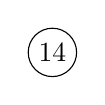
\begin{tikzpicture}[baseline=(n.base)]\node[draw,circle,inner sep=2pt] (n) {\unsure{14}};\end{tikzpicture}}}

\scanpage{12}
\mspage{30}
\margin{\unsure{1}}
\deleted{
\deleted{on a nécessairement} puisque ses composantes connexes sont ouvertes ($S$
étant localement noethérien). Mais alors on a nécessairement $Z=J_S$,
où $J$ est une partie de $I$, et on a \deleted{\unsure{donc}} donc $U=\varnothing$ ou $U=S$, suivant que $J$
est infini ou fini, ce qui donne la conclusion voulue.

\uline{Corollaire} 5.14. Soi\deleted{t}\inserted{ent} $S$ un préschéma localement noethérien et \uline{normal},
$P$ un $S$-préschéma \deleted{localement} constant tordu quasi-isotrivial. Alors les
composantes connexes de $P$ sont finies sur $S$.

Comme $P$ est étale sur $S$, on sait que $P$ est normal (SGA I 9.5.)
donc ses composantes \deleted{irréductibles} connexes sont ses composantes
irréductibles. On peut évidemment supposer $S$ connexe donc irréductible,
soit $s$ son point générique. Comme $R$ est plat sur $S$, ses points maximaux,
i.e. les points génériques $x_i$ des composantes irréductibles $R_i$ de $R$,
sont les points maximaux de $R_s$, et la fibre \deleted{\unsure{de R}} générique $R_{i\,s}$ de $R_i$
est la composante irréductible de $R_s$, adhérence de $x_i$ dans $R_s$. Or
$R_s$ étant étale sur $k(s)$, est somme disjointe de spectres \unsure{dr'extensions|d'extensions}
finies séparables de $k(s)$, donc \deleted{les} pour tout $i$, $R_{i\,s}$ est fini (en
fait, réduit à un seul point). Donc 5.13. s'applique et montre que
les $R_i$ sont finis sur $S$.

\uline{Remarque} 5.15. Le raisonnement s'applique, plus généralement, si on
suppose seulement $S$ géométriquement unibranche au lieu de normal, i.e.
que le morphisme \unsure{Canonique|canonique} $\widetilde S\longrightarrow S$, où $\widetilde S$ est le normalisé de $S_{\text{réd}}$,
est radiciel. Donc le théorème 5.16. ci-dessous est valable également
sous cette condition plus générale.

\uline{Théorème} 5.16. Soit $S$ un préschéma localement noethérien normal. Alors
tout groupe de type multiplicatif \deleted{\unsure{de type fini}} \inserted{et de type fini} sur $S$ \deleted{\unsure{local et en parti}}
est \uline{isotrivial}.
\inserted{\uline{On peut} supposer en effet \inserted{\figure{\begin{tikzpicture}[baseline=(n.base)]\node[draw,ellipse,inner sep=1pt] (n) {$S$ connexe, donc};\end{tikzpicture}}} $H$ de type constant $M$.}
Il suffit d'appliquer 5.13 . avec $P=\underline{\operatorname{Isom}}_{S\text{-gr}}(H,G)$, où $G=D_S(M)$,
}
\inserted{en raisonnant comme dans \unsure{5.10|5.14}. (ii)$\Longrightarrow$(i); \uline{on peut aussi} \unsure{appli-}\\
ou \deleted{\unsure{encore}} \unsure{5.11}. \deleted{\illegible{3}}, en utilisant \unsure{5.14} pour $R=D_S(\unsure{\check H|\check M})$.}
\margin{\unsure{5.11}.}
\margin{\figure{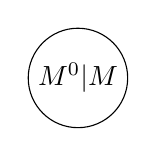
\begin{tikzpicture}[baseline=(n.base)]\node[draw,circle,inner sep=2pt] (n) {$\unsure{M^0|M}$};\end{tikzpicture}}}
\margin{\unsure{M}}
\margin{11}

\scanpage{13}
la deuxième \deleted{\unsure{se}} se ramène à:
\[
E_n={}_{f^n}E_{n+1}
\]
qui par $a_n)$ équivaut à $\supset$, donc à ceci

soit $x\in E_n$, $h\in A$, \deleted{$\unsure{f^nx}$} tels qu'il existe $\lambda\in A$, avec
\[
f^n(x,h)=\lambda(\xi_n,f)
\]
alors on a $h\in fA$. En effet, on aura
\[
f^nh=\lambda f\quad\text{d'où}\quad\lambda=f^{n-1}h,
\qquad(\text{\uline{car $f$ est $A$-régulier}})
\]
puis $f^nx=\lambda\xi_n$ \deleted{\unsure{ou $f^n$}} i.e.
\[
0=f^{n-1}h\xi_n,\quad\text{or}\quad
(\overbrace{f^{n-1}\xi_n}^{\eta_n})\in{}_fE_n\quad\text{par }a_n),
\]
\deleted{d'où} et ${}_fE_n\simeq A/fA=B$ par $b_n)$, \deleted{donc}
enfin par construction on a $\xi_n\notin{}_{f^{n-1}}E_n$ i.e.
\[
\deleted{\unsure{f^n}}\eta_n\ne0,\quad\text{donc}\quad
h\eta_n\unsure{=|\ne}0\ \Rightarrow\ h\in fA,\quad\text{cqfd.}
\]

Enfin, vérifions $c_n$, on a
\[
\begin{aligned}
E_{n+1}/fE_{n+1}
&=(E_n\times A)/f(E_n\times A)+A(\xi_n,f)\\
&\simeq(E_n/fE_n\times A/fA)/A(\bar\xi_n,\bar f)\\
&\simeq([B\times(B/gB)^{n-1}]\times B)/B(g,0,0)\\
&\simeq B/gB\times(B/gB)^{n-1}\times B\simeq B\times(B/gB)^n.
\end{aligned}
\]
\margin{12}

\scanpage{14}
\mspage{29}
\deleted{
images dans $S$ sont des parties $S_i$ à la fois ouvertes et fermées, et
elles recouvrent $S$. Si $S$ est connexe ou quasi-compact, il existe donc
un ensemble fini d'indices \deleted{\unsure{tel}} $i$ tels que les $S_i$ recouvrent $S$, soit
$S'$ la réunion des $P_i$ correspondants, \deleted{\unsure{qui est donc tel que}}\inserted{Alors}
$S'\unsure{-|\longrightarrow}S$ est fini étale surjectif, et posant
$P'=P\times_S S'=\underline{\operatorname{Isom}}_{S'\text{-gr}}(H',G')$, on voit que $P'$
a une section sur $S'$, donc il existe un isomorphisme de $S'$-groupes
$H'=H\times_S S'\xrightarrow{\sim}G'=G\times_S S'=D_{S'}(M)$, ce qui prouve que $S'$ splitte $H$. Le
cas où les composantes \deleted{irréductibles}\inserted{connexes} de $S$ sont \deleted{\unsure{connexes}} ouvertes se ramène
aussitôt au cas où $S$ est connexe. -- Remarquons d'ailleurs qu'on peut,
lorsque $H$ est de type fini sur $S$, \deleted{\unsure{connexe}} et de type constant, donner
\unsure{le|he} critère d'isotrivialité suivant (où il n'est plus nécessaire de faire
aucune restriction sur $S$): $R$ est réunion d'une \uline{suite} de parties à la
fois ouvertes et fermées finies sur $S$.

\uline{Lemme} 5.1\unsure{3|2}. Soient $S$ un préschéma localement noethérien et connexe,
$\unsure{R|P}$ un $S$-préschéma constant tordu quasi-isotrivial, $Z$ une partie à la fois
ouverte et fermée de $R$, telle qu'il existe un $s\in S$ tel que $Z_s$ soit fini.
Alors $Z$ est fini sur $S$.
\margin{$Z_s$}
\margin{$Z$}

\deleted{Oublions un instant que $S$ est supposé connexe, et}\inserted{Ne supposons pas d'abord $S$ connexe;}
soit $U$ l'ensemble
des $s\in S$ tels que $Z_s$ soit fini, nous allons prouver que $U$ est à la
fois ouvert et fermé, et que $Z|U$ est fini sur $U$. C'est là évidemment
un \deleted{énoncé} énoncé essentiellement équivalent à 5.1\unsure{3|2}. mais qui a l'avantage
d'être ``de nature locale'' sur $S$ pour la topologie étale (disons), ce
qui nous ramène au cas où $\unsure{P|R}$ est constant, i.e. de la forme $\unsure{I|K}_S$, où $I$ est
un ensemble. (NB l'hypothèse localement noethérienne n'est pas perdue
par un changement de base étale; c'est là où on utilise la quasi-isotrivialité
de $P$ sur $S$). On peut de plus supposer $S$ connexe, \deleted{mais alors}
}
\margin{13}

\scanpage{15}
On construit $E_{n+1}$ comme extension
de $A/fA$ par $E_n$, \deleted{\unsure{par}} déduite de l'extension
\unsure{standart|standard} \unsure{de} $A$ de $A/fA$ par $A$ par un homo
$A-E_n$ défini par un élément $\xi_n$ de $E_n$
(l'extension $E_{n+1}$ ne dépend que de $\xi_n\bmod fE_n$).
\diagram{\begin{tikzcd}[column sep=large]
0 \arrow[r,dash] & A \arrow[r,"f"] \arrow[d,"\xi"'] & A \arrow[r] \arrow[d] & A/fA \arrow[r,dash] \arrow[d,Rightarrow] & 0\\
0 \arrow[r,dash] & E_n \arrow[r] & E_{n+1} \arrow[r] & A/fA \arrow[r,dash] & 0
\end{tikzcd}}

Notons que \inserted{par $a_n)$} $fE_n\subset\deleted{f}{}_{f^{n-1}}E_n$ donc
\diagram{\begin{tikzcd}[column sep=small]
0 \arrow[r,dash] & {}_{f^{n-1}}E_n/fE_n \arrow[r] & E_n/fE_n \arrow[r] & E_n/{}_{f^{n-1}}E_n \arrow[r,dash] \arrow[d,phantom,"\rotatebox{90}{$\simeq$}"] & 0\\
&&& A/fA=B &
\end{tikzcd}}

Comme $g$ est \unsure{régulier} dans $B$,
\deleted{et \unsure{le premier homo de} \unsure{homo}}\inserted{tout homo}
($B$-linéaire) de $B+(B/gB)^{n-1}$ dans $B$ est de la
\deleted{première} forme $\lambda\operatorname{pr}_1$ $(\lambda\in B)$, et s'il
\deleted{\unsure{est}} est surjectif, $\lambda$ est inv. Donc l'isom
$c)$ \deleted{est}\inserted{peut être pris} compatible avec la structure
d'extension précédente [où ${}_{f^{n-1}}E_n/fE_n\simeq(B/gB)^{n-1}$]

Nous \unsure{choisirons|désirons} $\dot\xi_n=\deleted{\unsure{\bar\xi_n}}(\dot g,0)$. \deleted{Alors}

Vérifions les propriétés $a_{n+1})$, $b_{n+1})$, $c_{n+1})$.
La première résulte trivialement de $(a_n)$ et $fA/fA=0$
\margin{14}

\scanpage{16}
\mspage{28}
\deleted{
\uline{Lemme} 5.12. Soient $S$ un préschéma, $R$ un préschéma constant tordu sur $S$.
Alors tout sous-préschéma fermé \deleted{$\unsure{T|Z}$}\inserted{$Z$} de $R$ qui est
\deleted{de type fini}\inserted{quasi-compact} sur $S$,
est fini sur $S$.

En effet, on est ramené au cas où $R$ est constant, donc de la forme
$I_S$, où $I$ est un ensemble, donc réunion filtrante croissante des $J_S$, où
$J$ parcourt les parties finies de $I$. On peut supposer de plus $S$ affine,
alors \deleted{$\unsure{R|Z}$} $Z$ est quasi-compact, donc contenu dans un des $J_S$. Comme $J_S$
est fini sur $S$, il en est de même de $Z$.

Le lemme 5.12. établit déjà l'assertion entre parenthèses dans
5.11. (ii). \deleted{L'équivalence $(ii)\unsure{\Leftrightarrow|-}(iii)$ est}\inserted{L'implication $(ii)\Rightarrow(iii)$, et \unsure{llimplication|l'implication} inverse}
dans le cas $S$ localement
noethérien est alors claire. Prouvons que $(i)\Rightarrow(ii)$, pour ceci, soit
$S'\longrightarrow S$ un morphisme étale fini surjectif qui splitte $H$ donc $R$, de sorte
que $R'$ s'écrit \deleted{comme} $M_S=\deleted{\unsure{\sum}}\coprod_{m\in M}R'_m$, où \deleted{tous} les $R'_m$ sont des ouverts
disjoints de $R'$, \inserted{$S'$-}isomorphes à $S'$. Soit $g:R'\longrightarrow R$ la projection, qui est
un morphisme fini étale surjectif, \inserted{donc un morphisme ouvert et fermé;}
alors les $R_m=g(R'_m)$ sont des parties
à la fois ouvertes et fermées de $R$, et évidemment quasi-compacts sur $S$
puisque les $R_m$ le sont. \deleted{Enfin, prouvons $(ii)\unsure{-|\Rightarrow}(i)$}

Enfin, prouvons $(ii)\Rightarrow(i)$ lorsque $H$ est de type fini sur $S$,\inserted{$S$ quasi compact ou connexe.} Soit
$M$ son type, on peut écrire $M=\deleted{\unsure{N}}\underline{Z}^{,r}\times N$, où $r$ est un entier $\geq0$
et $N$ un groupe fini. Considérons le préschéma
\[
P=\underline{\operatorname{Isom}}_{S\text{-gr}}(H,G)\subset
\underline{\operatorname{Hom}}_{S\text{-gr}}(H,G)\unsure{=|\ne}Q
\]
où $G=D_S(M)$, cf 5.8. et 5.10. \deleted{Alors $Q$ est isomorphe} On a un isomorphis\unsure{me}
\[
Q\simeq\underline{\operatorname{Hom}}_{S\text{-gr}}(G,\underline{G}_m^{,r})\times
\underline{\operatorname{Hom}}_{S\text{-gr}}(G,N)\simeq R^r\times E,
\]
où $E=\underline{\operatorname{Hom}}_{S\text{-gr}}(G,N)$ est fini sur $S$. Il s'ensuit que $Q$ est
\deleted{réunion de}\inserted{réunion de sous-}préschémas à la fois ouverts et fermés $Q_i$ finis sur $S$. \deleted{De même, il
s'ensuit que}\inserted{Donc} $P$ est réunion \deleted{\unsure{d'un}} de \deleted{\unsure{présch}} sous-préschémas à la fois
ouverts et fermés $P_i$\inserted{$=P\cap Q_i$} finis sur $S$. Comme ils sont étales sur $S$, leurs
}
\margin{15}

\scanpage{17}
De plus, la construction donne un homo
\diagram{\begin{tikzcd}E_n\arrow[r,dash,"u_n"]&E_{n+1}\end{tikzcd}}
tel que l'homo correspondant
\[
u_n\otimes_A B:\quad\underset{Q_n}{E_n/fE_n}\ -\ \underset{Q_{n+1}}{E_{n+1}/fE_{n+1}}
\]
soit \uline{nul} sur $g(E_n/fE_n)$, et induise un
homo injectif de \inserted{\unsure{on note ainsi}} $\deleted{E_n/fE_n}\inserted{Q_n}\otimes_B B/gB$ dans
\deleted{\unsure{et définissant un homo injec} et $Q_{n+1}$ \unsure{appliquant} une base de}
de $Q_{n+1}\otimes^B B/gB$, \unsure{appliquant} une base sur
une base (on est dans modules libres).

Donc
\[
\begin{aligned}
\varinjlim_n Q_n&=\varinjlim_n Q_n\otimes_B B/gB\simeq\varinjlim_n(B/gB)^{n-1}\\
&\simeq(B/gB)^{(\mathbf N)}.
\end{aligned}
\]
Prenons donc
\[
M=\varinjlim_n E_n
\]
Alors $M$ satisfait aux conditions voulues.
\margin{16}

\scanpage{18}
\mspage{27}
\margin{27}
\deleted{
\uline{Corollaire} 5.9. Les foncteurs 5.7. induisent des anti-équivalences
quasi-inverses l'une de l'autre entre la catégorie des groupes de type
multiplicatif de type fini\inserted{$H$} sur $S$, et la catégorie des groupes constants
tordus à engendrement fini\inserted{$R$} sur $S$. Tout tel groupe $R$ est quasi-isotrivial.

\uline{Corollaire} 5.10. Soient $H,G$ deux \deleted{\unsure{de}} $S$-préschémas en groupes de type
multiplicatif et de type fini. Alors $\underline{\operatorname{Isom}}_{S\text{-gr}}(H,G)$ est représentable
par un sous-préschéma ouvert\inserted{et fermé} de $\underline{\operatorname{Hom}}_{S\text{-gr}}(H,G)$, et c'est un \deleted{\unsure{schéma}}
$S$-préschéma constant tordu. En particulier, $\underline{\operatorname{Aut}}_{S\text{-gr}}(H)$ est représentable
et est un groupe constant tordu (en général non commutatif) sur $S$.

Cela résulte de 5.8. et de Exp VIII\deleted{\unsure{.}} 1.6.

\uline{Proposition} 5.11. Soient $S$ un préschéma, $R$ un groupe constant tordu
sur $S$, $H=D_S(R)$ le groupe de type multiplicatif qu'il définit. Considérons les conditions suivantes:

(i) $H$ est isotrivial, (i.e. $R$ est isotrivial).

(ii) $R$ est \deleted{somme disjointe de}\inserted{réunion de} sous-préschémas\inserted{à la fois ouverts et fermés} $R_i$, qui sont quasi-compacts
(et alors nécessairement finis) sur $S$.

(iii) Les composantes connexes de $R$ sont finies sur $S$.

Alors $(i)\Rightarrow(ii)\Rightarrow(iii)$, on a $\inserted{(i)\Leftrightarrow}(ii)\Leftrightarrow(iii)$ si $S$ est localement
noethérien, enfin $(i)\Leftrightarrow(ii)$ si $R$ est \deleted{\unsure{de}} à engendrement fini i.e.
si $H$ est de type fini, \inserted{du moins si $S$ est quasi-compact ou si ses
composantes connexes sont ouvertes.}

\deleted{Démonstration. $(i)\unsure{-|\Rightarrow}(ii)$ Soit $S'-S$ fini étale surjectif qui
splitte $H$ donc $R$, de sorte que $R'$ est \unsure{somm}}

Décomposant d'abord $S$ en préschéma somme de préschémas $S_i$ sur chacun desquels $H$ est de type constant (cf Exp IX\deleted{\unsure{.}} 1), on
est ramené au cas où $H$ \deleted{est de} donc $R$ est de type constant. Nous aurons
besoin\deleted{\unsure{(pour (ii))}} d'un

\deleted{\uline{Lemme} 5.11.}
}
\margin{17}

\scanpage{19}
Théorème de

M. Artin sur $\mathrm{cd}$

\margin{\unsure{30|20}}
\margin{18}

\scanpage{20}
\uline{Théorèmes de M. Artin}

\uline{Th. 1} Soit $K$ une extension de \uline{type fini} de $\mathbb Q$,\inserted{$X$ un modèle.} Conditions
équivalentes:
\margin{suffit-il de degré de transcendance fini ??}

(i) $-1$ est une somme de carrés dans $K$

(i bis) $K$ n'admet pas de structure de corps ordonné

(i ter) $K$ n'est pas isomorphe à un sous-corps de $\mathbb R$

(ii) \deleted{Il existe un modèle} $X$ \deleted{de $K$ qui} n'a pas de pt simple réel.

\deleted{
(ii bis) Tout modèle $X$ de $K$ est sans point simple réel.

(ii ter) Il existe un modèle [propre] \deleted{sans point \unsure{simple}}\inserted{simple. sans} pt réel

(ii quater) Tout modèle (propre) simple est sans pts réels.
}

(ii bis) \deleted{(Si $X$ est un modèle)}
$\dim$\inserted{\figure{\begin{tikzpicture}[baseline=(n.base)]\node[draw,ellipse,inner sep=2pt] (n) {topologique};\end{tikzpicture}}}
$X(\mathbb R)<n=\text{\unsure{degré|degr} tr. }K/\mathbb Q$

(ii \unsure{ter}) $X(\mathbb R)$ est \deleted{contenu dans un fermé}\inserted{\unsure{rare} dans $X_C$ pour la} top. de Zariski.

(ii quater) (Si $X$ simple/$\mathbb Q$) \quad $X(\mathbb R)=\varnothing$

(iii) $\mathrm{cd}_2(K)<+\infty$

\deleted{\unsure{(ii bis)}}\inserted{(iii bis)}
(\uline{si} $X_{\unsure{\mathbb R|\mathbb Q}}$ \uline{simple sur} $\mathbb R$) \quad $\mathrm{cd}_2(X)<+\infty$

\uline{Corollaire} 1 Soit $X$ un préschéma de type fini sur $Z$
\deleted{\unsure{resp sur}}
\deleted{(resp sur $\mathbb Q$)} Conditions équivalentes:

(i) $X(\mathbb R)=\varnothing$

(ii) $\mathrm{cd}_2(X)<+\infty$

\deleted{(ii bis) $\mathrm{cd}_2(X)\leq2\dim X+1$ \quad (resp. $\leq2\dim X+2$)}

(iii) $\mathrm{cd}_2(X_{\mathbb Q})<+\infty$

\deleted{S'il en est ainsi, on a}

(iv) $\mathrm{cd}_2(X_{\mathbb R})<+\infty$

Alors
\[
\mathrm{cd}(X)<2\dim X+1,\qquad
\mathrm{cd}(X_{\mathbb Q})\leq2\dim X_{\mathbb Q}+1,
\qquad\mathrm{cd}(X_{\mathbb R})\leq2\dim X
\]
\margin{19}

\scanpage{21}
\figure{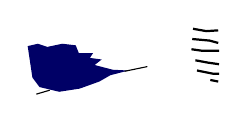
\begin{tikzpicture}[x=1cm,y=1cm]
\fill[blue!40!black] (0,.33)--(.13,.36)--(.25,.32)--(.44,.36)--(.61,.34)--(.65,.24)--(.83,.24)--(.79,.18)--(.94,.16)--(.85,.09)--(1.08,.03)--(1.28,.02)--(1.05,-.04)--(.91,-.12)--(.66,-.21)--(.4,-.25)--(.15,-.19)--(.06,-.07)--cycle;
\draw[thin] (1.23,.01)--(1.52,.07) (.11,-.28)--(.28,-.23);
\draw[thick] (2.1,.55)--(2.27,.52)--(2.42,.53) (2.09,.42)--(2.31,.4)--(2.42,.37) (2.08,.29)--(2.22,.27)--(2.43,.27) (2.13,.15)--(2.29,.12)--(2.43,.1) (2.15,.02)--(2.35,-.02)--(2.43,-.02) (2.32,-.1)--(2.42,-.12);
\end{tikzpicture}}

\rotatebox{180}{\begin{minipage}{.65\linewidth}
\uline{Def} \quad $\mathbf F$ sheaf on $X$ is

\deleted{$X$}
\end{minipage}}
\margin{20}

\scanpage{22}
\uline{Corollaire} 2 Soit $K$ extension de type fini de $\mathbb R$,
$X$ un modèle. Conditions équivalentes (i) (i bis) (ii) (ii bis)
(ii ter) (ii quater) (iii) (iii bis).
\deleted{(i) $-1$ une somme de carrés dans $K$}

\uline{Corollaire} 3 $X$ préschéma de type fini sur $\mathbb R$.

Conditions équivalentes

(i) $X(\mathbb R)=\varnothing$

(ii) $\mathrm{cd}_2(X)<+\infty$

\deleted{\unsure{Alors}} Lorsqu'il en est ainsi, alors pour \inserted{tt} faisceau
(étale) $F$ sur $X$, on a
\[
H^i(X,F)\simeq H^i(\underbrace{X(C)/\mathbb Z/2\mathbb Z}_{\text{topologie ordinaire}},F)
\]
et on a
\[
\mathrm{cd}_2(X)\leq2\dim X
\]

\uline{Théorème} 2 Soit $k$ un corps,\inserted{\figure{\begin{tikzpicture}[baseline=(n.base)]\node[draw,ellipse,inner sep=3pt] (n) {$r$ un \deleted{\unsure{entier}} \inserted{\unsure{nb} premier}};\end{tikzpicture}}}
\deleted{$k'$ une \unsure{e}}\inserted{Conditions} équivalentes

\margin{Conditions th. 2 \unsure{satisfaites} \unsure{pourvu que} \uline{l'une}
des conditions suiv. \unsure{ait lieu}
$\left\{\begin{array}{l}
\operatorname{car}k>0\\
r\ne2\\
-1\text{ somme de carrés}\\
\text{\unsure{non}}\ \mathrm{cd}_2k(\sqrt{-1})<+\infty]\\\relax
[\mathrm{cd}_r(k)<+\infty]
\end{array}\right.$}

\figure{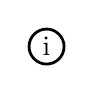
\begin{tikzpicture}[baseline=(n.base)]\node[draw,circle,inner sep=2pt,line width=1pt] (n) {i};\end{tikzpicture}}
Pour \unsure{tte|tt} extension de type fini $k'$ de $k$, on a
\[
\mathrm{cd}_r(k')=\mathrm{cd}_r(k)+\operatorname{deg\,tr}k'/k
\]

(i bis) Comme dessus, \deleted{$k'$ une extension quadratique}\inserted{avec $k'=k(\sqrt{-1})$ !}
\deleted{(et même $k'=k(\sqrt{-1})$ !)}

(ii) $k'$ contient un corps\inserted{$k_0$} de type fini sur le corps
premier, et tel que $\mathrm{cd}_r(k_0)<+\infty$, ou $\mathrm{cd}_2k(\sqrt{-1})=+\infty$

\figure{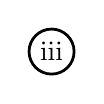
\begin{tikzpicture}[baseline=(n.base)]\node[draw,circle,inner sep=2pt,line width=1pt] (n) {iii};\end{tikzpicture}}
On n'est pas dans le cas suivant: $k$ est
ordonnable (\deleted{donc}\inserted{i.e.} de car $0$\inserted{et $-1$ n'est pas somme de carrés}), $r=2$,
\figure{\begin{tikzpicture}[baseline=(n.base)]\node[draw,ellipse,inner sep=4pt] (n) {$\mathrm{cd}_2(k(\sqrt{-1}))<+\infty$.};\end{tikzpicture}}
\inserted{[d'où $\mathrm{cd}_2(k)=+\infty$]}
\margin{21}

\scanpage{23}
\uline{Corollaire} $A$ anneau local \deleted{hensélien} noethérien
intègre, corps des fractions $K$, corps résiduel $k$.
Alors pour tt premier $r$, on a
\[
\mathrm{cd}_r(K)\geq\mathrm{cd}_r(k)+\dim A
\]
\deleted{[avec \uline{égalité} dans le cas $A$ hensélien \unsure{?}]}
\deleted{\inserted{\figure{\begin{tikzpicture}[baseline=(n.base)]\node[draw,ellipse,align=left,inner sep=3pt] (n) {et $A$ \unsure{Univ.} japonais\\\unsure{univ. caténaire}};\end{tikzpicture}}}}
\margin{\deleted{\unsure{à le}}}

sauf exception possible dans les cas suivants:

a) $r$ est la caractéristique de $K$\inserted{(égale caractéristique $>0$)}

b) $r=2$, \deleted{$A$ un anneau de \unsure{dim $1$}, $r=2$, Il existe}
\deleted{$A$ ``d'inégales caractéristiques'', \unsure{que} la caractéristique
résiduelle est $2$, \unsure{$r=$} un idéal premier $\mathfrak p\subset A$, \unsure{non nul}, avec $A/\mathfrak p$ de dim $1$.}
$\exists\ x\in\operatorname{Spec}(A)$ tel que $\kappa(x)$
soit ordonnable, et $\mathrm{cd}_2\kappa(x)(\sqrt{-1})$ soit fini
(corps réel \unsure{coulant|courant}).
\margin{\uline{Ex} $A=\mathbb R[x,y]/(x^2+y^2)$ \uline{\unsure{localisé}}}

\uline{NB.} Si $A$ est \uline{caténaire} et \uline{univ. japonais},
(ce que garantit le fait que les \unsure{lieux normaux}
des sous-schémas de $A$ sont ouverts), alors
\deleted{il suffit} on peut préciser\inserted{dans le cas b)}, \deleted{\unsure{à quel}} l'exception
possible par: $k$ lui-même ``corps réel \unsure{coulant|courant}''.
Enfin, lorsque $A$ est \uline{régulier},
cette exception elle-même est inoffensive, i.e.
on a l'inégalité annoncée, (pourvu qu'on ne
soit dans le cas a)].
\margin{cette restriction est-elle \unsure{inutile} ???}
\margin{22}

\scanpage{24}
Comparaison de topologies \unsure{\ldots}

Lemme de Cartan
\margin{4}
\margin{23}

\scanpage{25}
\uline{Lemme de Cartan}

$\unsure{\mathbb T|T}$ \deleted{\unsure{un}} site, \deleted{$S\in\unsure{\mathrm{Ob}\,T|T}$}

$F$ faisceau abélien sur $T$

$n\in\mathbb Z$

\deleted{$\mathcal U\inserted{\unsure{=(U_i^\alpha)}}$ famille \unsure{filtrante} croissante de rec. de $S$\inserted{\unsure{cofinale}},}

$\mathcal M$ sous-ens de $\operatorname{Ob}T$ \deleted{formé de}
\deleted{tt}
\inserted{\figure{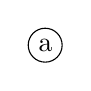
\begin{tikzpicture}[baseline=(n.base)]\node[draw,circle,inner sep=2pt] (n) {a};\end{tikzpicture}} $\mathcal M$ stable par produits finis}

On suppose \deleted{que}\inserted{\figure{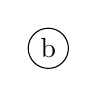
\begin{tikzpicture}[baseline=(n.base)]\node[draw,circle,inner sep=2pt] (n) {b};\end{tikzpicture}}}
pour tt $S\in\deleted{\unsure{\operatorname{Ob}T}}\inserted{\mathcal M}$, \deleted{\unsure{il existe}}
les \uline{recouvrements} de $S$ formés par des $\in\mathcal M$ sont
cofinaux pour les rec [il suffit \unsure{$=$}, qu'ils
suffisent à effacer \deleted{$\unsure{H^q(S,)}$} tt classe
de $H^q(\unsure{S|U},F)$, $0<q\leq n$.].

\margin{\figure{\begin{tikzpicture}[x=1cm,y=1cm]
\draw[thin] (.1,4.6) .. controls (1.2,4.4) and (2.2,4.35) .. (3.1,4.5);
\draw[line width=.6pt] (0,4.4) .. controls (-.08,3.5) and (.18,2.8) .. (.08,2.2);
\draw[thin] (.06,4.42) .. controls (.14,4.1) and (.1,3.9) .. (.03,3.6);
\draw[thin] (.1,2.15) .. controls (.18,1.2) and (.26,.4) .. (.26,0);
\draw[thin] (2.2,.5)--(4.3,2.6);
\node at (.18,2.75) {$\unsure{*}$};
\end{tikzpicture}}}

Conditions équivalentes

(i) $\forall S\in\mathcal M$, $H^i(S,F)=0$ pour $0<i\leq n$

(ii) $\forall S\in\mathcal M$, \deleted{\unsure{tout}} et tt rec.\inserted{$\mathcal U$} de $S$
formé par des $S_i\in\mathcal M$, on a
\[
\check H^i(\mathcal U,F)=0\quad\text{pour }0<i\leq n
\]

(iii) $\forall S\in\mathcal M$, on a
\[
\varinjlim_{\mathcal U}\check H^i(\mathcal U,F)=0\quad\text{pour }0<i\leq n
\]
où $\mathcal U$ varie sur les rec de $S$ formés
d'objets $\in\mathcal M$
\margin{\figure{\begin{tikzpicture}\draw (0,2.2)--(0,1.8);\draw (.04,.6)--(.07,0);\end{tikzpicture}}}
\margin{24}

\scanpage{26}
\mspage{\unsure{35|55}}
tel que $A$ soit séparé et complet pour la topologie $J$-adique. Sous ces conditions:

(i) Le foncteur $F\rightsquigarrow\widehat F$ de la catégorie des Modules localement libres
sur $U'$ dans la catégorie des Modules localement libres sur $\widehat U'$ est
pleinement fidèle.

(ii) Pour tout Module localement libre $\underline F$ sur $\widehat U'$, il existe un Module
cohérent $F$ sur $\unsure{U'|V'}$ (pas nécessairement localement libre, hélas), et un
isomorphisme $\widehat F\simeq\underline F$.

Il reste seulement à prouver (ii), grâce à 5.9. Or d'après \unsure{ceytte|cette}
remarque, et exposé IX 2.1. il s'ensuit que $\underline F$ est induit par un Module
cohérent $\underline G$ sur $\widehat X'$. D'après le théorème \deleted{de comparaison et} d'existence\inserted{EGA $\overline{\underline{\mathrm{III}}}$}
5.1.4., $\underline G$ est de la forme $\widehat F$, où $F$ est cohérent sur $X$, d'où la conclusion.

\uline{Remarques} 5.1\unsure{0|1}.\inserted{$1^{\mathrm o})$} Utilisant 5.10.\inserted{, 4.7.}
\deleted{et des hypothèses convenables de}
une hypothèse convenable, disant que certains anneaux locaux des fibres
géométriques de $X'\quad S'$ sont ``purs'' resp. \unsure{parafactoriels|Parafactoriels}, on doit pouvoir
obtenir des énoncés disant \deleted{\unsure{que}} que le foncteur $Z'\rightsquigarrow\widehat Z'$ de la catégorie
des revêtements étales de $X'$ dans la catégorie des revêtements étales de
$\widehat X'$ \deleted{est} (ou ce qui revient au même, de $X'_0$) est \deleted{pleinement fidèle} une
équivalence de catégories, resp. que le foncteur $\underline L\rightsquigarrow\widehat{\underline L}$ de la catégorie
des Modules inversibles sur $X'$ dans la catégorie des Modules inversibles
sur $\widehat X'$ est une équivalence. Utilisant des résultats récents de MURRE,
il est probable que l'on doit pouvoir en déduire des théorèmes d'existence
\deleted{pour} des schémas de Picard pour \deleted{des}\inserted{certains} schémas algébriques \deleted{propres} \uline{non}
\uline{propres}. \deleted{\unsure{voir}} De façon générale, l'élimination d'hypothèses de propreté
dans divers théorèmes d'existence, notamment de représentabilité de
foncteurs comme les foncteurs de Hilbert, ou de Picard etc, à l'aide
\margin{25}

\scanpage{27}
On a (i)$\Rightarrow$(ii) par suite spectrale
\[
H^{\unsure{p+q|\ast}}(S,F)\Longleftarrow H^p(\mathcal U,H^q(F))=E_2^{pq}
\]
l'hyp (i) implique $E_2^{pq}=0$ pour $0<q\leq n$, \uline{et}
\deleted{l'hyp préliminaire que $E_2^{\unsure{p0|pq}}=0$ pour $q=0$,}
\margin{\figure{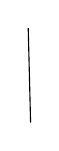
\begin{tikzpicture}\draw (0,1.2)--(.03,0);\end{tikzpicture}}}
d'où
\[
H^i(S,F)\xleftarrow{\sim}H^i(\mathcal U,F)\quad\text{pour }i\leq n
\]
et par suite $H^i(\mathcal U,F)\simeq0\deleted{\unsure{H^i}}$ pour $0<i\leq n$.

(ii)$\Rightarrow$(iii) trivial

(iii)$\Rightarrow$(i) par récurrence sur $n$. C'est
\deleted{\unsure{trivial}}\inserted{vide} si $n\leq0$. Supposons $n>0$, et l'assertion
prouvée pour $n'<n$. \deleted{Alors on a déjà, par
l'hyp de récurrence
\[
E_2^{pq}=0\quad\text{si }0<q<n
\]}
\inserted{Regardons}
\[
H^{\unsure{p+q|\ast}}(S,F)\Longleftarrow\varinjlim_{\mathcal U}H^p(\mathcal U,H^q(F))=E_2^{pq}
\]
Par hyp de récurrence, on a
\[
\text{a)}\quad E_2^{pq}=0\quad\text{si }0<q<n
\]
\deleted{de plus, $\unsure{E_2^{p0}=0}$, \unsure{on a que}}
Par hyp (iii), on a
\[
\text{b)}\quad E_2^{pq}=0\quad\text{si }q=0,\ 0<p\leq n
\]
Enfin on sait par \deleted{\unsure{la}}\inserted{l'hyp. préliminaire}
\[
\text{a)}\quad E_{\unsure{2|4}}^{pq}=0\quad\text{si }p\unsure{\geq|=}0,\ q>0
\]
\margin{\figure{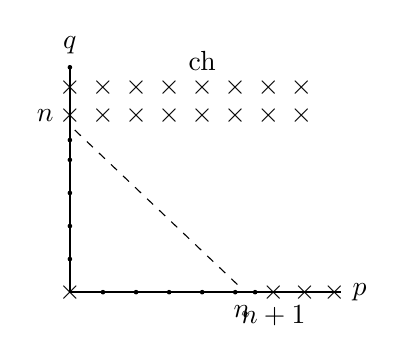
\begin{tikzpicture}[x=.42cm,y=.42cm]
\draw[line width=.8pt] (0,6.8)--(0,0)--(8.2,0);
\node[above] at (0,6.9) {$q$};\node[right] at (8.25,0) {$p$};
\node[left] at (-.2,5.35) {$n$};\node[below] at (5.2,-.12) {$n$};\node[below] at (6.15,-.12) {$n+1$};
\node at (4,7) {\unsure{ch}};
\foreach \y in {1,2,3,4,4.6,6.8}{\fill (0,\y) circle (.07);}
\foreach \x in {1,2,3,4,5,5.6}{\fill (\x,0) circle (.07);}
\foreach \x in {0,1,2,3,4,5,6,7}{\node at (\x,5.35) {$\times$};\node at (\x,6.2) {$\times$};}
\foreach \x in {0,6.15,7.1,8}{\node at (\x,0) {$\boldsymbol\times$};}
\draw[dashed] (.15,4.9)--(5.15,.15);
\end{tikzpicture}}}
On trouve alors $E_2^{pq}=0$ si $p+q=n$, d'où
$H^n(S,F)=0$, \unsure{qfd.|cqfd.}
\margin{26}

\scanpage{28}
\mspage{9}
Posons
\[
\text{(2.5)}\qquad\underline S=\operatorname{gr}_{\mathcal J}\underline O_{X'}
=\coprod_{k\in\underline{\underline N}}\mathcal J^k/\mathcal J^{k+1}
\]
\[
\text{(2.6)}\qquad\operatorname{gr}_{\mathcal J}(\underline F)
=\coprod_{k\in\underline{\underline N}}\mathcal J^k\underline F/\mathcal J^{k+1}\underline F
\]
\[
\text{(2.7)}\qquad\underline K^i=R^if_*(\operatorname{gr}_{\mathcal J}(\underline F))
=\coprod_{k\in\underline{\underline N}}R^if_*(\mathcal J^k\underline F/\mathcal J^{k+1}\underline F),
\]
il est clair que $\underline K^i$ est muni d'une structure de $\underline S$-Module
gradué.

\uline{Théorème 2.1.} Supposons que $\underline K^i$ soit un $\underline S$-Module gradué
\uline{de type fini} pour $i=n-1,i=n,i=n+1$, alors:

(i) $R^nf_*(F)$ est cohérent

(ii) l'homomorphisme $\unsure{\psi|\varphi}_n$, (2.3), est un isomorphisme
topo\inserted{l}ogique\inserted{, La filtration naturelle du deuxième membre
de (2.3.) est $\mathcal J$-bonne.}

(iii) le système projectif des $R^nf_*(F_k)$ vérifie
la condition de Mittag-Leffler uniforme.

La démonstration est très facile à partir de
E.G.A.$0_{\mathrm{III}}$.13.7.7.\inserted{(cf. E.G.A. III 3.4.2.)}, à condition de rectifier comme suit
le texte page 78:

\uline{Supprimer}

\begin{tabular}{ll}
ligne 6 & `` et $(R^{n+1}T(A_k))_{k\in\underline{\underline Z}}$ ''\\[1ex]
ligne 13 & `` et $p+q=n+1$''\\[1ex]
ligne 23 & `` et pour $n+1$''.
\end{tabular}

\uline{Théorème 2.2.} Soit $A$ un anneau adique noethérien et soit
$I$ un idéal de définition de $A$.\inserted{Soit $T$ une partie fermée de $X'=\operatorname{Spec}(A)$.}
Supposons que $I$ soit engendré par un $t\in A$. Reprenons les notations (1.31)\inserted{,}(1.32) et
(1.33). Soit $\underline F$ un $\underline O_{\widehat X}$-Module cohérent. Posons
\[
\text{\unsure{(2.8)|(2.89)}}\qquad F_0=\underline F/\mathcal J\underline F,
\]
où $\mathcal J=t\underline O_{\widehat X}$ est un idéal de définition de $\widehat X$.
\margin{27}

\scanpage{29}
\uuline{Lemme} Notations $\unsure{\mathbb T|T},F,n,\mathcal M$ comme dans le
lemme de Cartan.\inserted{Considérons les} Conditions \deleted{équivalentes}

(i) $\forall S\in\mathcal M$,
\figure{\begin{tikzpicture}[baseline=(n.base)]\node[draw,ellipse,inner sep=5pt] (n) {$\deleted{\unsure{H}}\varinjlim_{\mathcal U}H^i(\mathcal U,F)$};\end{tikzpicture}}
$\simeq H^i(S,F).\qquad i\leq n$

[$\mathcal U$ parcourt les rec. de $S$ formés de $S_i\in\mathcal M$,]

(ii) $\forall S\in\mathcal M$, \deleted{et tt rec. $\mathcal U$ de $S$ formé
d'objets de $\unsure{S|\mathcal M}$, et tt élément:}
\[
\varinjlim_{\mathcal U}H^p(\mathcal U;H^q(F))=0\quad\text{pour }
\deleted{\unsure{0<q\leq n|0<p+q\leq n}\text{ et }q\ne0}\inserted{0<q\leq n\unsure{+1}}
\]

(iii)
\[
\varinjlim_{\mathcal U}H^p(\mathcal U,\overline H^q(F))=0\quad\text{pour }0<q\leq n\unsure{+1}
\quad\deleted{\text{et }\unsure{p|q}=0}
\]
où on pose\inserted{pour $T\in\mathcal M$,}
\[
\overline H^q(F)(T)=\varinjlim_{\mathcal V}H^q(\mathcal V,T),
\]
$\mathcal V$ parcourant les rec. de $T$ formés d'objets de $\mathcal M$.

(ii bis) $\forall S\in\mathcal M$, $\mathcal U$ rec. de $S$ par des $U_i\in\mathcal M$,
et $\unsure{\gamma|\zeta}\in\unsure{C^p|Z^p}(\mathcal U,H^q(F))$,
\deleted{($\unsure{p\geq0},p+q\leq n-1,\ q\ne0$)}\inserted{$0<q\leq n$}
il existe $\mathcal U'$ rec. de $S$ par des $U_i\in\mathcal M$, majorant $\mathcal U$,
\deleted{\unsure{tel que le}} et $\mathcal U'\unsure{-|\longrightarrow}\mathcal U$, tel que l'image de
$\unsure{\gamma|\zeta}$ dans $C^p(\mathcal U',H^q(F))$ soit nulle.

(iii bis) \deleted{$\unsure{\Leftarrow|\Leftrightarrow}$} Comme (ii bis), mais $H^qF$,
remplacé par $\overline H^q(F)$.

Mais on a
\diagram{\begin{tikzcd}[column sep=large,row sep=small]
\deleted{\text{(ii bis)}}\arrow[r,Rightarrow]\arrow[d,Rightarrow]&\deleted{\text{(ii)}}\arrow[d,Rightarrow]\\
{}\arrow[r,dash]&{}
\end{tikzcd}}
\diagram{\begin{tikzcd}[column sep=large,row sep=small]
\text{(ii bis)}\arrow[r,Leftrightarrow]\arrow[d,Rightarrow]&\text{(iii bis)}\\
\text{(ii \deleted{\unsure{bis}})}\arrow[r,Leftrightarrow]\arrow[d,Rightarrow]&\text{(iii)}\\
\text{(i)}&
\end{tikzcd}}
\margin{\figure{\begin{tikzpicture}[x=1cm,y=1cm]
\draw (0,4.8)--(.02,4.1);
\draw[thin] (.15,3.7)..controls(-.3,3.6)and(-.2,3.5)..(-.16,3.1)--(-.04,2.2)..controls(.1,2.2)and(.3,2.25)..(.48,2.3);
\draw[thin] (.1,1.8)..controls(-.1,1.8)and(-.08,1.7)..(-.1,1.5)--(-.1,.1)..controls(-.08,0)and(.06,0)..(.2,0);
\end{tikzpicture}}}
\margin{28}

\scanpage{30}
\mspage{8}
\margin{29}

(ii) L'homomorphisme canonique
\[
\deleted{H^i(X,F)}\ R^i\widehat f(\widehat F)\qquad \lim R^if(F_m)
\]
est un isomorphisme pour $i\quad n$, un monomorphisme pour $i=n+1$ \deleted{\unsure{;}}

Démonstration. On se ramène aussitôt au cas où $S$ est affine, et à prouver alors le

\uline{Corollaire} 2.2. Sous les conditions de 2.1. supposons de plus $S$ affine.
Alors :

(i) L'homomorphisme canonique
\[
H^i(X,F)\qquad H^i(\widehat X,\widehat F)
\]
est un isomorphisme pour $i\quad n$, un monomorphisme pour $i=n$.

(ii) L'homomorphisme canonique
\[
H^i(\widehat X,\widehat F)\qquad \lim H^i(X_m,F_m)
\]
est un isomorphisme pour $i\quad n$, un monomorphisme pour $i=n+1$.

\deleted{Pour \unsure{Démontrer|démontrer}} Quitte à remplacer $\underline O_X(1)$ par une puissance tensorielle, et $t$ par une puissance de $t$, on peut supposer $\underline O_X(1)$ très ample relativement à $S$. D'autre part, $t$ donc $t^m$ étant $F$-régulier, la multiplication par $t^m$, considéré comme homomorphisme de $F(-m)$ dans $F$, est injectif, donc on a pour tout $m\quad 0$ une suite exacte :
\diagram{\begin{tikzcd}[column sep=large]
(14) & 0 & F(-m)\arrow[r,phantom,"t^m"] & F & F_m & 0,
\end{tikzcd}}
d'où une suite exacte de cohomologie
\diagram{\begin{tikzcd}[column sep=large]
H^i(X,F(-m)) & H^i(X,F) & H^i(X,F_m) & H^{i+1}(X,F(-m)).
\end{tikzcd}}
Or en vertu de 1.5. on a $H^i(X,F(-m))=0$ pour $i\quad n$, et $m$ grand, ce qui prouve le

\uline{Lemme} 2.3. \deleted{\unsure{On}} Pour $m$ grand, l'homomorphisme canonique
\[
H^i(X,F)\qquad H^i(X_m,F_m)
\]
est bijectif si $i\quad n$, injectif si $i=n$.

Cela montre que pour $i\quad n$, le système projectif $(H^i(X_m,F_m))_m$

\scanpage{31}

\unsure{la s. s.} suite spectrale
\[
H^{\unsure{*|p+q}}(S,F)\Longleftarrow\varinjlim_U H^p(U,H^q(F))=E_2^{pq}.
\]
et
\[
E_2^{pq}=0\quad\text{si}\quad p=0,\ q>0.
\]

\unsure{Car} \deleted{\unsure{prouve}}\inserted{implique} déjà $(ii)\Rightarrow(i)$, Or moyennant $(i)$, $(ii)$ et $(iii)$ sont équivalents, donc $(ii)\Rightarrow(iii)$. De même trivialement $(ii\text{ bis})\Rightarrow(ii)$ et $(iii\text{ bis})\Rightarrow(iii)$, \deleted{et \unsure{on a} $(ii)\Rightarrow(i)$}\inserted{donc $(ii\text{ bis})\Rightarrow(i)$}, et \deleted{\unsure{que nous}} moyennant $(i)$, $(ii\text{ bis})$ et $(iii\text{ bis})$ sont équivalents, \unsure{i.e. on a} $(ii\text{ bis})\Rightarrow(iii\text{ bis})$. Tout sera fait

\margin{\diagram{\begin{tikzcd}[column sep=small,row sep=large]
& (ii)\arrow[dl,Rightarrow]\arrow[dr,Rightarrow] && (ii\text{ bis})\arrow[ll,Rightarrow]\arrow[dr,Rightarrow]\arrow[d,phantom,"{\deleted{\Downarrow}}"] & \\
(i) && (iii)\arrow[ll,Rightarrow]\arrow[r,phantom,"{\deleted{\Longrightarrow}}"] & \deleted{\unsure{(iii\text{ bis})}} & (iii\text{ bis})\arrow[ll,Rightarrow]
\end{tikzcd}}}

si nous prouvons que $(iii)\Rightarrow(i)$. Récurrence sur $n$. Si $n\leq0$, c'est vide. Supposons $n>0$, et que c'est prouvé pour $n'<n$. Donc on sait déjà que
\[
H^i(F)=\overline H^i(F)\quad\text{pour}\quad\uuline{i<n}\quad\deleted{\text{et}}
\]
\deleted{\unsure{faut le prouver pour} $i=n$} sur des arguments $\in\mathcal M$, donc
\[
E_2^{pq}=0\quad\text{si}\quad\deleted{p+q\leq n+1\text{ et }q\ne0}\inserted{0<q\leq\uline{n-1}}.
\]
\deleted{Donc} Mais

\margin{\figure{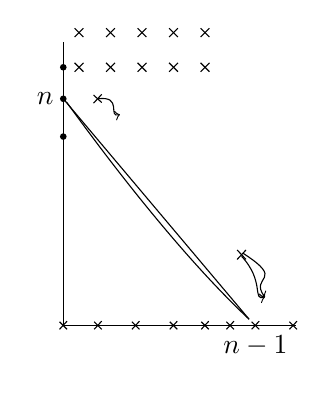
\begin{tikzpicture}[x=0.8cm,y=0.8cm]
\draw (0,0)--(3.7,0);\draw (0,0)--(0,4.5);
\foreach \x in {0,0.55,1.15,1.75,2.25,2.65,3.05,3.65}{\draw (\x-0.06,-0.06)--(\x+0.06,0.07);\draw (\x-0.06,0.06)--(\x+0.06,-0.06);}
\foreach \y in {3.0,3.6,4.1}{\fill (0,\y) circle (1.2pt);}
\foreach \x in {0.25,0.75,1.25,1.75,2.25}{\foreach \y in {4.1,4.65}{\draw (\x-0.07,\y-0.07)--(\x+0.07,\y+0.07);\draw (\x-0.07,\y+0.07)--(\x+0.07,\y-0.07);}}
\draw (0,3.6)--(2.95,0.1);\draw (0.05,3.55)..controls (1.1,2.1) and (2.1,0.9)..(2.95,0.1);
\node[left] at (0,3.6) {$\unsure{n}$};\node[below] at (3.05,0) {$n-1$};
\draw[->] (0.55,3.6)..controls (0.95,3.65) and (0.7,3.3)..(0.9,3.35);
\draw (0.48,3.53)--(0.61,3.67);\draw (0.48,3.66)--(0.61,3.54);
\draw[->] (2.85,1.15)..controls (3.55,0.7) and (2.95,0.8)..(3.2,0.45);
\draw[->] (2.83,1.1)..controls (3.2,0.7) and (3.0,0.4)..(3.2,0.45);
\draw (2.76,1.05)--(2.9,1.2);\draw (2.76,1.2)--(2.9,1.05);
\end{tikzpicture}}}

la suite spectrale donne
\[
\deleted{\unsure{H^n(S,F)}\simeq}
\]
\[
\varinjlim_U H^n(U,F)\simeq H^n(S,F)
\]
\deleted{\unsure{d'où encore}} \deleted{\unsure{H^n(F)}} cqfd.

\uline{Schéma logique} \unsure{Résumons} les \unsure{4} implications ci-contre, plus le fait que
\[
(i)\Longrightarrow[(ii)\Rightarrow(iii)\text{ et }(ii\text{ bis})\Leftrightarrow(iii\text{ bis})]
\]
\margin{\diagram{\begin{tikzcd}[column sep=small,row sep=small]
(ii\text{ bis})\arrow[d,Rightarrow]\arrow[rr,phantom,"{\deleted{\unsure{\Longleftrightarrow}}}"] && (iii\text{ bis})\arrow[d,Rightarrow]\\
(ii)\arrow[dr,Rightarrow] && (iii)\arrow[dl,Rightarrow]\\
& (i) &
\end{tikzcd}}}
\margin{30}

\scanpage{32}
\mspage{9}
\margin{31}

est essentiellement constant, \deleted{pour} à fortiori satisfait la condition de Mittag-Leffler, donc (compte tenu que $\widehat F=\lim F_m$) on conclut (ii) par EGA $0_{\mathrm{III}}$ 13/3. D'autre part (i) en résulte trivialement, compte tenu de 2.3.

\uline{Corollaire} 2.4. Soient $f:X\quad S$ un morphisme projectif et plat, avec $S$ localement noethérien, $\underline O_X(1)$ un Module inversible sur $X$, ample rela\deleted{\unsure{ti}}tivement à $S$, $t$ une section de ce module, qui soit $\underline O_X$-régulière, $Y$ \deleted{un} le sous-\unsure{préschéma|présbhéma} des zéros de $t$, $\widehat X$ le complété formel de $X$ le long de $Y$. On suppose que pour tout $s\quad S$, $X_s$ est de profondeur $\quad1$ (resp. de profondeur $\quad2$) en ses points fermés. Alors pour tout voisinage ouvert $U$ de $Y$, le foncteur
\[
F\qquad\widehat F
\]
de la catégorie des Modules cohérents localement libres sur $U$, dans la catégorie des Modules cohérents localement libres sur $\widehat X$, est fidèle (resp. pleinement fidèle, i.e. la condition \deleted{(Lef)} de Lefschetz (Lef) de l'exposé X N°2 est vérifiée).

Introduisons \deleted{le Module} pour deux Modules localement libres $F$ et $G$ sur $U$ le Module
\[
H=\underline{\operatorname{Hom}}_{\underline O_U}(F,G),
\]
on est ramené à prouver que l'homomorphisme canonique
\[
H^0(U,H)\qquad H^0(\widehat X,\widehat H)
\]
est injectif (resp. bijectif). Or les Modules $H_t$ sont de profondeur $\quad1$ (resp. $\quad2$) aux points fermés de $X_y$, on peut donc appliquer 2.1., qui implique la conclusion 2.4. dans le cas où $U=X$. Dans le cas d'un $U$ quelconque, on note que la question est locale sur $S$, donc on peut supposer $S$ affine. Alors tout Module cohérent sur $X$ est quotient d'un Module cohérent localement libre, (puisque $\underline O_X(1)$ est un Module inversible absolument ample sur $X$). Comme \unsure{He|le} Module dual $H'=\operatorname{Hom}(H,\underline O_U)$

\scanpage{33}

Calculs divers.

(\unsure{cup directs} \unsure{formule de} etc)

\margin{4 p \unsure{polycop} \unsure{!|1} $+3+6$}
\margin{32}

\scanpage{35}
\mspage{\unsure{5|S}}
\margin{GRÖTHENDIECK.}

\begin{center}
UNIVERSITÉ DE PARIS

\figure{\begin{tikzpicture}\draw (-.4,0)--(-.06,0);\fill (0,0) circle (.7pt);\draw (.06,0)--(.4,0);\end{tikzpicture}}

ÉCOLE NORMALE SUPÉRIEURE

\figure{\begin{tikzpicture}\draw (-.4,0)--(-.06,0);\fill (0,0) circle (.7pt);\draw (.06,0)--(.4,0);\end{tikzpicture}}

45, RUE D'ULM

ODÉON 06$\cdot$45

\figure{\begin{tikzpicture}\draw (-.4,0)--(-.06,0);\fill (0,0) circle (.7pt);\draw (.06,0)--(.4,0);\end{tikzpicture}}
\end{center}

\margin{\uuline{Th 1}}
Soit $E$ un ensemble simplicial, \deleted{\unsure{un}} $G$ un groupe discret qui opère sur $E$ p\deleted{\unsure{a}}ar des Transformations simpliciales, $B$\inserted{$=E/G$} l'ensemble simplicial quotient, \deleted{\unsure{alors}} $p:E\to B$ la projection canonique. Si $E$ est connexe, l'image de $p_*:\pi_1(E)\to\pi_1(B)$ est un sous groupe distingué de $\pi_1(B)$, et $\pi_1(B)/\operatorname{im}p_*(\pi_1(E))=G/S$, où $S$ est le sous groupe (distingué) de $G$ engendré par les stabilisateurs des sommets de $E$, et $E/S$ est le revêtement \deleted{\unsure{universel}} de $B$ \inserted{correspondant à l'image de $p_*(\pi_1(E))$}

\margin{\figure{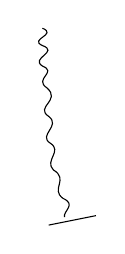
\begin{tikzpicture}[x=.4cm,y=.4cm]
\draw (0,5.6)..controls (.5,5.4) and (-.45,5.25)..(0,5.05)..controls (.55,4.85) and (-.4,4.65)..(0,4.4)..controls (.5,4.2) and (-.3,4)..(.15,3.7)..controls (.6,3.3) and (-.25,3.1)..(.2,2.8)..controls (.6,2.5) and (-.15,2.2)..(.25,1.95)..controls (.65,1.7) and (.05,1.4)..(.35,1.1)..controls (.85,.8) and (.25,.5)..(.65,.2)..controls (1.1,0) and (.65,-.2)..(.7,-.4);
\draw (.2,-.65)--(1.7,-.35);
\end{tikzpicture}}}

\uuline{Déf.} une arête de $E$ est un 1-simplexe de $E$ muni d'un signe $+$ ou $-$. Si $\sigma$ est un 1-simplexe, on pose
\[
\unsure{d_1|\partial_1}(+\sigma)=\partial_1(\sigma),\quad
\partial_0(+\sigma)=\partial_0(\sigma),\quad
\partial_1(-\sigma)=\partial_0(\sigma),\quad
\partial_0(-\sigma)=\partial_1(\sigma).
\]
Un chemin est une suite\inserted{d'arêtes} $\gamma=(\gamma_1,\ldots\gamma_n)$ telle que $\partial_1(\gamma_{i+1})=\partial_0(\gamma_i)$. On pose $\partial_1(\gamma)=\partial_1(\gamma_1)$ et $\partial_0(\gamma)=\partial_0(\gamma_n)$. Un \deleted{\unsure{point}}\inserted{sommet} de base $x_0$ étant fixé dans $E$, un lacet est un chemin $\gamma$ tel que $\partial_1(\gamma)=\partial_0(\gamma)=x_0$. 2 Chemins $\gamma$ et $\gamma'$ sont homotopes si leurs réalisations géométriques sont homotopes modulo leurs extrémités. Cette relation d'équivalence est compatible avec la loi de composition « mise bout à bout » des chemins, et est engendrée par les suivantes :
\margin{34}

\scanpage{36}
\begin{center}
UNIVERSITÉ DE PARIS

\figure{\begin{tikzpicture}\draw (-.4,0)--(-.06,0);\fill (0,0) circle (.7pt);\draw (.06,0)--(.4,0);\end{tikzpicture}}

ÉCOLE NORMALE SUPÉRIEURE

\figure{\begin{tikzpicture}\draw (-.4,0)--(-.06,0);\fill (0,0) circle (.7pt);\draw (.06,0)--(.4,0);\end{tikzpicture}}

45, RUE D'ULM

ODÉON 06$\cdot$45

\figure{\begin{tikzpicture}\draw (-.4,0)--(-.06,0);\fill (0,0) circle (.7pt);\draw (.06,0)--(.4,0);\end{tikzpicture}}
\end{center}

\deleted{Soit $E$ \deleted{un ensemble simplicial} un C-W-Complexe, $G$ un groupe discret, opérant sur $E$ par des transformations qui préservent la décomposition cellulaire, $B=E/G$ l'\deleted{ensemble} C-W-Complexe quotient de $E$}

\uline{Lemme 1} : $\forall x$ sommet de $E$, $\beta$ chemin de $B$ tel que $\unsure{d_1|\partial_1}(\beta)=p(x)$,
\[
\exists\gamma\text{ chemin de }E\text{ tel que }\partial_1(\gamma)=x\text{ et }p(\gamma)=\beta
\]
\uuline{Dém} Il suffit de le voir si $\beta$ est une arête. Soit $\lambda$ une arête de $B$ telle que $p\lambda=\beta$. On a \deleted{$\unsure{\partial}$} $p(\partial_1\lambda)=\partial_1(p\lambda)=\partial_1\beta=p(x)$, d'où $\exists g\deleted{\unsure{g_0}}\in G$, $x=g.\partial_1\lambda$, et $\gamma=g\lambda$ répond à la question

\uline{Lemme 2} : l'image de $p_*:\pi_1(E)\to\pi_1(B)$ est un sous groupe distingué de $\pi_1(B)$

\uuline{Dém} : Soit $\gamma$ un lacet de \deleted{$\unsure{B}$} $E$, $\beta$ un lacet de $B$, $\lambda$ un chemin de $E$ tel que $\partial_1(\lambda)=x_0$ et $p_*(\lambda)=\beta$. On a $p(\partial_0\lambda)=\partial_0\beta=b_0=px_0$, d'où $\partial_0\lambda=gx_0$, et le lacet $(\lambda,g\gamma,-\lambda)$ se projette en $(\beta,p(\gamma),-\beta)$ ce qui démontre le lemme 2.

\uline{Définition de $\chi:G\to\pi_1(B)/\operatorname{Im}\pi_1(E)$ quand $E$ connexe}.

Pour Tout $g\in G$, soit $\gamma$ un chemin de $E$ tel que $\partial_1(\gamma)=x_0$, $\partial_0(\gamma)=gx_0$. \deleted{\unsure{$\chi(g)$ la classe de}} $p(\gamma)$ est un lacet de $B$, soit $\chi(g)$ sa classe dans $\pi_1(B)/\operatorname{im}\pi_1(E)$. Elle ne dépend pas du chemin $\gamma$ choisi, car, si $\gamma'$ est un autre chemin, $(\gamma,-\gamma')$ est un lacet de $B$, et \deleted{$\unsure{p(\gamma)=p(\gamma')}$} $p(\gamma)$ et $p(\gamma')$ ont même classe mod l'image de $\pi_1(E)$.
\margin{35}

